\chapter{Results \& Discussions}

In this chapter, we present and analyze the results obtained from the implementation and testing of the integrated controller and compliant power supply for USB Power Delivery. The primary objective of this research was to design a robust and efficient system capable of managing power delivery in compliance with the USB PD 3.1 specifications.

The results are organized into several sections, each focusing on different aspects of the system’s performance. We begin with an overview of the simulation results, highlighting key metrics such as power efficiency, response time, and compliance with USB PD standards. This is followed by a detailed discussion of the hardware implementation results, including the challenges encountered and the solutions devised to address them.

Furthermore, we compare the performance of our design with existing solutions, emphasizing the improvements and innovations introduced in this work. The chapter concludes with a critical analysis of the results, discussing their implications for future research and potential applications in real-world scenarios.

By systematically presenting and discussing the findings, this chapter aims to provide a comprehensive understanding of the effectiveness and reliability of the proposed design, thereby contributing valuable insights to the field of USB Power Delivery systems.

\section{Synthesis}

\begin{table}[H]
\centering
\caption{Post Synthesis Area Report}
\begin{tabular}{|l|r|r|r|r|l|}
\hline
\textbf{Instance} & \textbf{Cells} & \textbf{Cell Area} & \textbf{Net Area} & \textbf{Total Area} & \textbf{Wireload} \\ \hline
usb\_pd\_top & 4997 & 13178 & 0 & 13178 & \textless none\textgreater (D) \\ \hline
\quad usb\_pd\_phy\_wr\_u0 & 1729 & 4415 & 0 & 4415 & \textless none\textgreater (D) \\ \hline
\quad \quad crc32\_u0 & 218 & 471 & 0 & 471 & \textless none\textgreater (D) \\ \hline
\quad \quad bmc\_encoder\_u0 & 47 & 127 & 0 & 127 & \textless none\textgreater (D) \\ \hline
\quad \quad enc\_enc4b5b\_u0 & 26 & 36 & 0 & 36 & \textless none\textgreater (D) \\ \hline
\quad usb\_pd\_phy\_rd\_u0 & 1389 & 3915 & 0 & 3915 & \textless none\textgreater (D) \\ \hline
\quad \quad crc32\_u0 & 218 & 471 & 0 & 471 & \textless none\textgreater (D) \\ \hline
\quad \quad bmc\_decoder\_u0 & 102 & 241 & 0 & 241 & \textless none\textgreater (D) \\ \hline
\quad \quad dec\_4b5b\_u0 & 23 & 34 & 0 & 34 & \textless none\textgreater (D) \\ \hline
inc\_add\_322\_32\_8 & 53 & 100 & 0 & 100 & \textless none\textgreater (D) \\ \hline
cc\_line\_u0 & 18 & 45 & 0 & 45 & \textless none\textgreater (D) \\ \hline
\end{tabular}
\label{table:syn_data}
\end{table}
(D) = wireload is default in technology library

Table \ref{table:syn_data} provides a detailed breakdown of the post-synthesis area report for the USB Power Delivery (USB PD) controller. This table lists various instances within the design, such as usb\_pd\_top, usb\_pd\_phy\_wr\_u0, and crc32\_u0, along with their respective cell counts and areas. The CellArea column indicates the total area occupied by the cells in each instance, while the NetArea column shows the area used by the interconnections between these cells. The TotalArea column sums up the cell and net areas, providing a comprehensive view of the space utilization for each instance. Notably, the usb\_pd\_top instance has the highest cell count and area, reflecting its complexity and central role in the design. This detailed area report is crucial for understanding the spatial efficiency of this design and identifying potential areas for optimization.


\begin{table}[H]
\centering
\caption{Post Synthesis Power Consumption Data}
\begin{tabular}{|l|r|r|r|r|}
\hline
\textbf{Instance} & \textbf{Cells} & \textbf{Leakage(nW)} & \textbf{Dynamic(nW)} & \textbf{Total Power(nW)} \\ \hline
usb\_pd\_top & 4997 & 793.488 & 787926.862 & 788720.350 \\ \hline
\quad usb\_pd\_phy\_wr\_u0 & 1729 & 263.105 & 251567.330 & 251830.435 \\ \hline
\quad \quad crc32\_u0 & 218 & 30.430 & 44552.993 & 44583.423 \\ \hline
\quad \quad bmc\_encoder\_u0 & 47 & 7.873 & 5948.908 & 5956.782 \\ \hline
\quad \quad enc\_enc4b5b\_u0 & 26 & 2.283 & 1862.917 & 1865.200 \\ \hline
\quad usb\_pd\_phy\_rd\_u0 & 1389 & 229.996 & 233341.012 & 233571.008 \\ \hline
\quad \quad crc32\_u0 & 218 & 30.374 & 42808.180 & 42838.554 \\ \hline
\quad \quad bmc\_decoder\_u0 & 102 & 14.867 & 7937.039 & 7951.907 \\ \hline
\quad \quad dec\_4b5b\_u0 & 23 & 2.059 & 1041.678 & 1043.737 \\ \hline
inc\_add\_322\_32\_8 & 53 & 6.805 & 1048.890 & 1055.695 \\ \hline
cc\_line\_u0 & 18 & 2.763 & 5245.805 & 5248.569 \\ \hline
\end{tabular}
\label{table:power_syn}
\end{table}

Table \ref{table:power_syn} in your thesis presents the Post Synthesis Power Consumption Data for various instances within the USB Power Delivery (USB PD) system. This table is crucial as it provides insights into the power efficiency of your design. Each instance, such as usb\_pd\_top, usb\_pd\_phy\_wr\_u0, and crc32\_u0, is listed with its corresponding power consumption metrics: Leakage Power, Dynamic Power, and Total Power. For example, the usb\_pd\_top instance has a total power consumption of 788,720.350 nW, with 793.488 nW attributed to leakage and 787,926.862 nW to dynamic power. This detailed breakdown helps in identifying power-hungry components and optimizing the design for better power efficiency.

\section{Optimisation}
\begin{table}[H]
\centering
\caption{Post Optimisation Area Report}
\begin{tabular}{|l|r|r|r|r|l|}
\hline
\textbf{Instance} & \textbf{Cells} & \textbf{Cell Area} & \textbf{Net Area} & \textbf{Total Area} & \textbf{Wireload} \\ \hline
usb\_pd\_top & 4998 & 13148 & 0 & 13148 & \textless none\textgreater (D) \\ \hline
\quad usb\_pd\_phy\_wr\_u0 & 1722 & 4406 & 0 & 4406 & \textless none\textgreater (D) \\ \hline
\quad \quad crc32\_u0 & 215 & 469 & 0 & 469 & \textless none\textgreater (D) \\ \hline
\quad \quad bmc\_encoder\_u0 & 47 & 127 & 0 & 127 & \textless none\textgreater (D) \\ \hline
\quad \quad enc\_enc4b5b\_u0 & 22 & 34 & 0 & 34 & \textless none\textgreater (D) \\ \hline
\quad usb\_pd\_phy\_rd\_u0 & 1391 & 3907 & 0 & 3907 & \textless none\textgreater (D) \\ \hline
\quad \quad crc32\_u0 & 215 & 469 & 0 & 469 & \textless none\textgreater (D) \\ \hline
\quad \quad bmc\_decoder\_u0 & 102 & 243 & 0 & 243 & \textless none\textgreater (D) \\ \hline
\quad \quad dec\_4b5b\_u0 & 23 & 33 & 0 & 33 & \textless none\textgreater (D) \\ \hline
inc\_add\_322\_32\_8 & 53 & 100 & 0 & 100 & \textless none\textgreater (D) \\ \hline
cc\_line\_u0 & 18 & 45 & 0 & 45 & \textless none\textgreater (D) \\ \hline
\end{tabular}

\label{table:area_syn_data}
\end{table}
(D) = wireload is default in technology library

Table \ref{table:area_syn_data} provides a detailed breakdown of the area occupied by various components of the USB Power Delivery (USB PD) system after optimization. This table is crucial for understanding how the design has been refined to improve space efficiency. The optimization process has slightly reduced the total area for most instances, reflecting efforts to minimize the silicon footprint while maintaining functionality.

\begin{table}[H]
\centering
\caption{Post Optimisation Power Consumption Report}
\begin{tabular}{|l|r|r|r|r|}
\hline
\textbf{Instance} & \textbf{Cells} & \textbf{Leakage(nW)} & \textbf{Dynamic(nW)} & \textbf{Total Power(nW)} \\ \hline
usb\_pd\_top & 4998 & 759.540 & 216164.601 & 216924.141 \\ \hline
\quad usb\_pd\_phy\_wr\_u0 & 1722 & 256.107 & 75630.159 & 75886.266 \\ \hline
\quad \quad crc32\_u0 & 215 & 29.822 & 12512.385 & 12542.206 \\ \hline
\quad \quad bmc\_encoder\_u0 & 47 & 7.993 & 1615.830 & 1623.823 \\ \hline
\quad \quad enc\_enc4b5b\_u0 & 22 & 1.947 & 526.591 & 528.539 \\ \hline
\quad usb\_pd\_phy\_rd\_u0 & 1391 & 224.780 & 62714.504 & 62939.284 \\ \hline
\quad \quad crc32\_u0 & 215 & 29.747 & 8283.382 & 8313.129 \\ \hline
\quad \quad bmc\_decoder\_u0 & 102 & 15.063 & 3131.209 & 3146.272 \\ \hline
\quad \quad dec\_4b5b\_u0 & 23 & 1.638 & 302.191 & 303.829 \\ \hline
inc\_add\_322\_32\_8 & 53 & 6.074 & 614.177 & 620.251 \\ \hline
cc\_line\_u0 & 18 & 2.844 & 1824.601 & 1827.445 \\ \hline
\end{tabular}
\label{table:power_opt}
\end{table}

This \ref{table:power_opt} provides a detailed breakdown of the power consumption for various instances in the USB Power Delivery (USB PD) system after optimization. In \ref{table:power_syn}, the total power consumption for the usbpdtop instance is 788,720.350 nW. This value comprises both dynamic power (787,926.862 nW) and leakage power (793.488 nW). However, in the optimized Table \ref{table:power_opt}, we observe significant reductions:

\begin{enumerate}
    \item The total power consumption for usb\_pd\_top is now only 216,924.141 nW. This substantial reduction indicates improved efficiency and performance post-optimization.
    \item The dynamic power for usb\_pd\_top has decreased to 216,164.601 nW. This reduction in dynamic power signifies better energy utilization.
    \item The leakage power for usb\_pd\_top is slightly lower at 759.540 nW. Even minor reductions in leakage power contribute to overall efficiency gains.
\end{enumerate}
In summary, the optimized design achieves remarkable power savings, enhancing the USB PD system’s performance.


%\section{Floorplan and Placement}

\section{CTS}
\begin{table}[H]
\centering
\caption{Clock Tree Balancer Configuration for skew\_group sys\_clk/sdc\_cons}
\begin{tabular}{|l|r|}
\hline
\textbf{Clock Tree Balancer Configuration} & \textbf{Value} \\ \hline
Sources & pin sys\_clk \\ \hline
Total number of sinks & 1161 \\ \hline
Delay constrained sinks & 1161 \\ \hline
Non-leaf sinks & 0 \\ \hline
Ignore pins & 0 \\ \hline
Skew target & 0.101 ns \\ \hline
Insertion delay target & 0.300 ns \\ \hline
\end{tabular}
\label{table:clock_tree_balancer}
\end{table}
Table \ref{table:clock_tree_balancer} outlines the parameters used to balance the clock distribution in your USB Power Delivery controller design. The clock tree is a critical component in digital circuits, ensuring that the clock signal reaches all parts of the circuit simultaneously to maintain synchronization. The table lists the source pin as sys\_clk, indicating the primary clock input. It also shows the total number of sinks as 1161, which refers to the number of endpoints that receive the clock signal. The delay-constrained sinks are also 1161, meaning all sinks must meet specific timing constraints. 

There are no non-leaf sinks or ignore pins, simplifying the clock tree structure. The skew target is set to 0.101 ns, representing the maximum allowable difference in arrival times of the clock signal at different sinks. The insertion delay target is 0.300 ns, indicating the desired delay from the clock source to the sinks. This configuration aims to achieve precise and efficient clock distribution, crucial for the performance and reliability of design.
\begin{table}[H]
\centering
\caption{Clock Tree Legalization - Histogram}
\begin{tabular}{|l|r|}
\hline
\textbf{Movement ($\mu$m)} & \textbf{Number of cells} \\ \hline
[0, 0.371) & 163 \\ \hline
[0.371, 0.742) & 1 \\ \hline
[0.742, 1.113) & 0 \\ \hline
[1.113, 1.484) & 5 \\ \hline
[1.484, 1.855) & 0 \\ \hline
[1.855, 2.226) & 38 \\ \hline
[2.226, 2.597) & 0 \\ \hline
[2.597, 2.968) & 2 \\ \hline
[2.968, 3.339) & 0 \\ \hline
[3.339, 3.71) & 1 \\ \hline
\end{tabular}
\label{table:clock_tree_histogram}
\end{table}
Table \ref{table:clock_tree_histogram} provides a detailed breakdown of the movement of cells during the clock tree legalization process. This process ensures that the clock distribution network is optimized for minimal skew and jitter. The table categorizes the movement of cells into different ranges, measured in micrometers (\(\mu m\)). For instance, 163 cells moved within the range of 0 to 0.371 \(\mu m\), indicating minimal adjustment was needed. Only one cell moved between 0.371 and 0.742 \(\mu m\), and no cells moved in the next range. The table continues to show that five cells moved between 1.113 and 1.484 \(\mu m\), and 38 cells moved between 1.855 and 2.226 \(\mu m\). The remaining ranges have very few cells, indicating that most cells required minimal movement to achieve optimal clock distribution. This histogram helps in understanding the extent of adjustments made to ensure efficient clock signal distribution across the chip.
\begin{table}[H]
\centering
\caption{Clock Tree Layer Assignment (Top/Trunk High-Fanout Routes)}
\begin{tabular}{|l|c|c|c|c|c|}
\hline
\textbf{Layer} & \textbf{Pre-Route} & \textbf{Post-Route} & \textbf{R (Ohm $\mu$m$^{-1}$)} & \textbf{C (fF $\mu$m$^{-1}$)} & \textbf{RC (fs $\mu$m$^{-2}$)} \\
\hline
M2 & 0.000$\mu$m & 9.890$\mu$m & 3.808 & 0.173 & 0.660 \\
M3 & 809.555$\mu$m & 837.000$\mu$m & 3.965 & 0.175 & 0.694 \\
M4 & 659.425$\mu$m & 626.495$\mu$m & 3.808 & 0.173 & 0.657 \\
PLA & 100.000\% & 99.329\% & - & - & - \\
\hline
\end{tabular}
\label{table:clock_tree_layer_assignment}
\end{table}
Table \ref{table:clock_tree_layer_assignment} provides a detailed breakdown of the Clock Tree Layer Assignment for the top/trunk high-fanout routes in your USB Power Delivery controller design. This table is crucial for understanding how the clock signal is distributed across different metal layers in the chip, ensuring minimal skew and jitter.

The table lists the lengths of the clock routes before and after routing for each metal layer (M2, M3, M4). For example, M2 has a pre-route length of 0.000 \(\mu m\) and a post-route length of 9.890 \(\mu m\). It also includes the resistance and capacitance values for each layer, which are essential for calculating the RC delay. For instance, M2 has a resistance of 3.808 Ohm/\(\mu m\) and a capacitance of 0.173 fF/\(\mu m\).


\begin{table}[H]
\centering
\caption{Clock Tree Layer Assignment (Leaf Routes)}
\begin{tabular}{|l|c|c|c|c|c|}
\hline
\textbf{Layer} & \textbf{Pre-Route} & \textbf{Post-Route} & \textbf{R (Ohm / $\mu$m)} & \textbf{C (fF / $\mu$m)} & \textbf{RC (fs $\mu$m$^{-2}$)} \\
\hline
M2 & 0.000$\mu$m & 98.415$\mu$m & 3.808 & 0.173 & 0.660 \\
M3 & 3311.515$\mu$m & 3242.600$\mu$m & 3.965 & 0.175 & 0.694 \\
M4 & 3045.165$\mu$m & 3156.615$\mu$m & 3.808 & 0.173 & 0.657 \\
M5 & 0.000$\mu$m & 2.600$\mu$m & 3.965 & 0.175 & 0.694 \\
PLA & 100.000\% & 98.446\% & - & - & - \\
\hline
\end{tabular}
\label{table:clock_tree_layer_assignment_leaf}
\end{table}

Table \ref{table:clock_tree_layer_assignment_leaf} provides detailed information about the assignment of clock tree layers for leaf routes in the design1. The table lists the pre-route and post-route lengths of the clock tree on different metal layers (M2, M3, M4, and M5), along with their respective resistance, capacitance, and RC delay product (RC).


\section{Routing}
\begin{table}[H]
\centering
\caption{Pre-route Setup Mode Analysis}
\begin{tabular}{|l|r|r|r|}
\hline
\textbf{Setup mode} & \textbf{all} & \textbf{reg2reg} & \textbf{default} \\ \hline
\textbf{WNS (ns)} & 1.305 & 1.305 & 2.578 \\ \hline
\textbf{TNS (ns)} & 0.000 & 0.000 & 0.000 \\ \hline
\textbf{Violating Paths} & 0 & 0 & 0 \\ \hline
\textbf{All Paths} & 1180 & 1172 & 1109 \\ \hline
\end{tabular}
\label{table:pre_setup_analysis}
\end{table}
Table \ref{table:pre_setup_analysis} focuses on the setup mode analysis before routing. Here are the key metrics:
\begin{enumerate}
    \item \textbf{Worst Negative Slack (WNS)}: Indicates the most critical timing violation. A positive value of 1.305 ns suggests no violations.
    \item \textbf{Total Negative Slack (TNS)}: Represents the sum of all negative slacks. A value of 0 ns indicates no timing violations.
    \item \textbf{Violating Paths}: Indicates the number of paths failing to meet timing requirements. Here, it’s 0, indicating that all paths meet the timing constraints.
\end{enumerate}

\begin{table}[H]
\centering
\caption{Pre-route Hold Mode Analysis}
\begin{tabular}{|l|r|r|r|}
\hline
\textbf{Hold mode} & \textbf{all} & \textbf{reg2reg} & \textbf{default} \\ \hline
\textbf{WNS (ns)} & 0.060 & 0.060 & 1.856 \\ \hline
\textbf{TNS (ns)} & 0.000 & 0.000 & 0.000 \\ \hline
\textbf{Violating Paths} & 0 & 0 & 0 \\ \hline
\textbf{All Paths} & 1180 & 1172 & 1109 \\ \hline
\end{tabular}
\label{table:pre_hold_analysis}
\end{table}
Table \ref{table:pre_hold_analysis} focuses on the hold mode analysis before routing. Here are the key metrics:
\begin{enumerate}
    \item \textbf{Worst Negative Slack (WNS)}: A value of 0.060 ns indicates minimal timing violations.
    \item \textbf{Total Negative Slack (TNS)}: Remains at 0 ns, confirming no cumulative timing violations.
    \item \textbf{Violating Paths}: Again, 0 violating paths, meeting hold timing requirements.
\end{enumerate}
\begin{table}[H]
\centering
\caption{Post- route Setup Mode Analysis}
\begin{tabular}{|l|c|c|c|}
\hline
\textbf{Setup mode} & \textbf{all} & \textbf{reg2reg} & \textbf{default} \\
\hline
\textbf{WNS (ns)} & 3.533 & 3.533 & 5.321 \\ \hline
\textbf{TNS (ns)} & 0.000 & 0.000 & 0.000 \\ \hline
\textbf{Violating Paths} & 0 & 0 & 0 \\ \hline
\textbf{All Paths} & 1180 & 1172 & 1109 \\ \hline
%\hline
\end{tabular}
\label{table:post_setup_mode_analysis}
\end{table}
Now let’s look at the setup mode analysis after routing (Table \ref{table:post_setup_mode_analysis}):
\begin{enumerate}
    \item \textbf{Worst Negative Slack (WNS)}: A significant increase to 3.533 ns mainly due to added RC, indicating no setup timing violations.
    \item \textbf{Total Negative Slack (TNS)}: Still at 0 ns, ensuring no cumulative timing violations.
    \item \textbf{Violating Paths}: No violating paths, demonstrating compliance with setup timing requirements.
\end{enumerate}

\begin{table}[H]
\centering
\caption{Pre-route Hold Mode Analysis}
\begin{tabular}{|l|r|r|r|}
\hline
\textbf{Hold mode} & \textbf{all} & \textbf{reg2reg} & \textbf{default} \\ \hline
\textbf{WNS (ns)} & 0.068 & 0.065 & 1.956 \\ \hline
\textbf{TNS (ns)} & 0.000 & 0.000 & 0.000 \\ \hline
\textbf{Violating Paths} & 0 & 0 & 0 \\ \hline
\textbf{All Paths} & 1180 & 1172 & 1109 \\ \hline
\end{tabular}
\label{table:post_hold_analysis}
\end{table}
Finally, the hold mode analysis after routing (Table \ref{table:post_hold_analysis}):
\begin{enumerate}
    \item \textbf{Worst Negative Slack (WNS)}: A slight increase to 0.068 ns, still minimal timing violations.
    \item \textbf{Total Negative Slack (TNS)}: Remains at 0 ns, confirming no cumulative hold timing violations.
    \item \textbf{Violating Paths}: None, meeting hold timing requirements post-routing.
\end{enumerate}

These tables collectively demonstrate that this design meets both setup and hold timing requirements, ensuring robust performance and reliability.

\section{Physical Verification}
\subsection{SPEF Coverage}
\textbf{Standard Parasitic Exchange Format (SPEF)} is a file format used to describe the parasitic resistance and capacitance of interconnects in an integrated circuit. Accurate SPEF coverage is crucial for ensuring the reliability and performance of the design.

\textbf{Annotation to Verilog Netlist: 100\%}

This indicates that the parasitic information has been fully annotated to the Verilog netlist. The Verilog netlist is a textual representation of the circuit, describing the components and their connections. Full annotation means that every net in the Verilog netlist has corresponding parasitic data, ensuring that the simulation and analysis can account for all parasitic effects.

\textbf{Annotation to Physical Netlist: 100\%}

This signifies that the parasitic data has been completely annotated to the physical netlist. The physical netlist includes detailed information about the physical layout of the circuit, such as the placement of components and routing of interconnects. Full annotation here ensures that the physical design tools can accurately model the parasitic effects, leading to more precise timing and power analysis.

\vspace{10pt}
\textbf{Importance of 100\% Coverage}

\begin{enumerate}
    \item \textbf{Accuracy}: Ensures that all parasitic effects are considered, leading to more accurate simulations and analyses.
    \item \textbf{Reliability}: Helps in identifying potential issues related to parasitic resistance and capacitance, which can affect the performance and reliability of the circuit.
    \item \textbf{Optimization}: Provides a complete dataset for optimization tools to improve the design’s performance, power consumption, and area.
\end{enumerate}

\subsection{Top Level Netlist Check}
\begin{table}[h]
    \centering
    \caption{Port connected to core instances}
    \begin{tabular}{|l|c|}
        \hline
        \textbf{Port name} & \textbf{\# of connections} \\
        \hline
        cc2\_debug & 3 \\
        cc1\_debug & 3 \\
        cc2\_out & 1 \\
        cc1\_out & 1 \\
        cc\_oen & 1 \\
        cc2\_in & 3 \\
        cc1\_in & 3 \\
        sys\_nrst & 67 \\
        sys\_clk & 31 \\
        \hline
        \textbf{Ports connected to core instances} & \textbf{9} \\
        \hline
    \end{tabular}
        \label{tab:port_connections}
\end{table}
\textbf{The Top Level Netlist Check} is a crucial step in verifying the integrity and correctness of the netlist, which is a detailed description of the electronic circuit. This section ensures that the design is free from common issues that could affect its functionality.

\textbf{Floating Ports}: 0

This indicates that there are no floating ports in the design. A floating port is a port that is not connected to any signal or component, which can lead to unpredictable behavior. Having zero floating ports ensures that all ports are properly connected, enhancing the reliability of the design.

\textbf{Ports Connect to Multiple Pads}: 0

This means that no ports are connected to multiple pads. A port connected to multiple pads can cause signal conflicts and integrity issues. Ensuring that each port is connected to a single pad helps maintain signal clarity and prevents potential errors.

\textbf{Ports Connected to Core Instances}

This section lists the ports that are connected to core instances, along with the number of connections for each port. Core instances refer to the main functional blocks within the design. The breakdown of the connections is seen in table \ref{tab:port_connections}.

\vspace{10pt}

\textbf{Importance of Top Level Netlist Check Verification:} 

\begin{enumerate}
    \item Ensures that all ports are correctly connected, preventing floating ports and multiple connections that can cause design failures.
    \item Signal Integrity: Maintains the integrity of signals by ensuring proper connections, which is vital for the correct operation of the circuit.
    \item Design Reliability: Enhances the overall reliability and robustness of the design by identifying and rectifying potential issues early in the design process.
\end{enumerate}

\subsection{High Fanout Nets}

\begin{table}[h]
    \centering
    \caption{High Fanout Nets}
    \label{tab:high_fanout_net}
    \begin{tabular}{|l|}
        \hline
        \textbf{Net Name} \\ \hline
        usb\_pd\_phy\_wr\_u0/crc32\_u0/n\_185 \\ \hline
        usb\_pd\_phy\_rd\_u0/crc32\_u0/n\_185 \\ \hline
        n\_1418 \\ \hline
        n\_307 \\ \hline
        sys\_nrst \\ \hline
        FE\_OFN102\_sys\_nrst \\ \hline
        usb\_pd\_phy\_wr\_u0/FE\_OFN111\_n\_175 \\ \hline
        usb\_pd\_phy\_wr\_u0/FE\_OFN112\_n\_177 \\ \hline
        FE\_OFN187\_n\_308 \\ \hline
        FE\_OFN188\_n\_308 \\ \hline
        FE\_OFN189\_n\_308 \\ \hline
        FE\_OFN214\_n\_291 \\ \hline
        FE\_OFN217\_n\_297 \\ \hline
        FE\_OFN218\_n\_297 \\ \hline
        FE\_OFN221\_n\_307 \\ \hline
    \end{tabular}
\end{table}

A \textbf{High Fanout Net} refers to a net that drives a large number of inputs. High fanout can lead to increased load on the driving cell, which can affect the performance and timing of the circuit. Table \ref{tab:high_fanout_net} list the high fanout nets in the design.

\begin{enumerate}
    \item \textbf{usb\_pd\_phy\_wr\_u0/crc32\_u0/n\_185  and usb\_pd\_phy\_rd\_u0/crc32\_u0/n\_185:} These nets are part of the CRC32 module within the USB PD PHY write and read units. High fanout in these nets indicates that the CRC32 calculation results are being used extensively across the design.
    \item \textbf{n\_1418 and n\_307:} These are generic nets with high fanout, likely used in multiple places within the design. The specific function would depend on the context within the netlist.
    \item \textbf{sys\_nrst and FE\_OFN102\_sys\_nrst:} The sys\_nrst net is the system reset signal, which is typically distributed widely across the design to ensure all components can be reset. The FE\_OFN102\_sys\_nrst is likely a buffered or optimized version of the system reset signal to manage the high fanout.
    \item \textbf{usb\_pd\_phy\_wr\_u0/FE\_OFN111\_n\_175  and usb\_pd\_phy\_wr\_u0/FE\_OFN112\_n\_177:} These nets are part of the USB PD PHY write unit, indicating signals that are distributed to multiple destinations within the write unit.
    \item \textbf{FE\_OFN187\_n\_308, FE\_OFN188\_n\_308, FE\_OFN189\_n\_308:} These nets are likely optimized or buffered versions of a signal (n\_308) to manage the high fanout. Buffering helps in maintaining signal integrity and timing.
    \item \textbf{FE\_OFN214\_n\_291, FE\_OFN217\_n\_297, FE\_OFN218\_n\_297, FE\_OFN221\_n\_307:} Similar to the previous nets, these are likely buffered or optimized versions of signals (n\_291, n\_297, n\_307) to handle the high fanout.
\end{enumerate}

\section{Power Supply}

\begin{figure}[H]
    \centering
    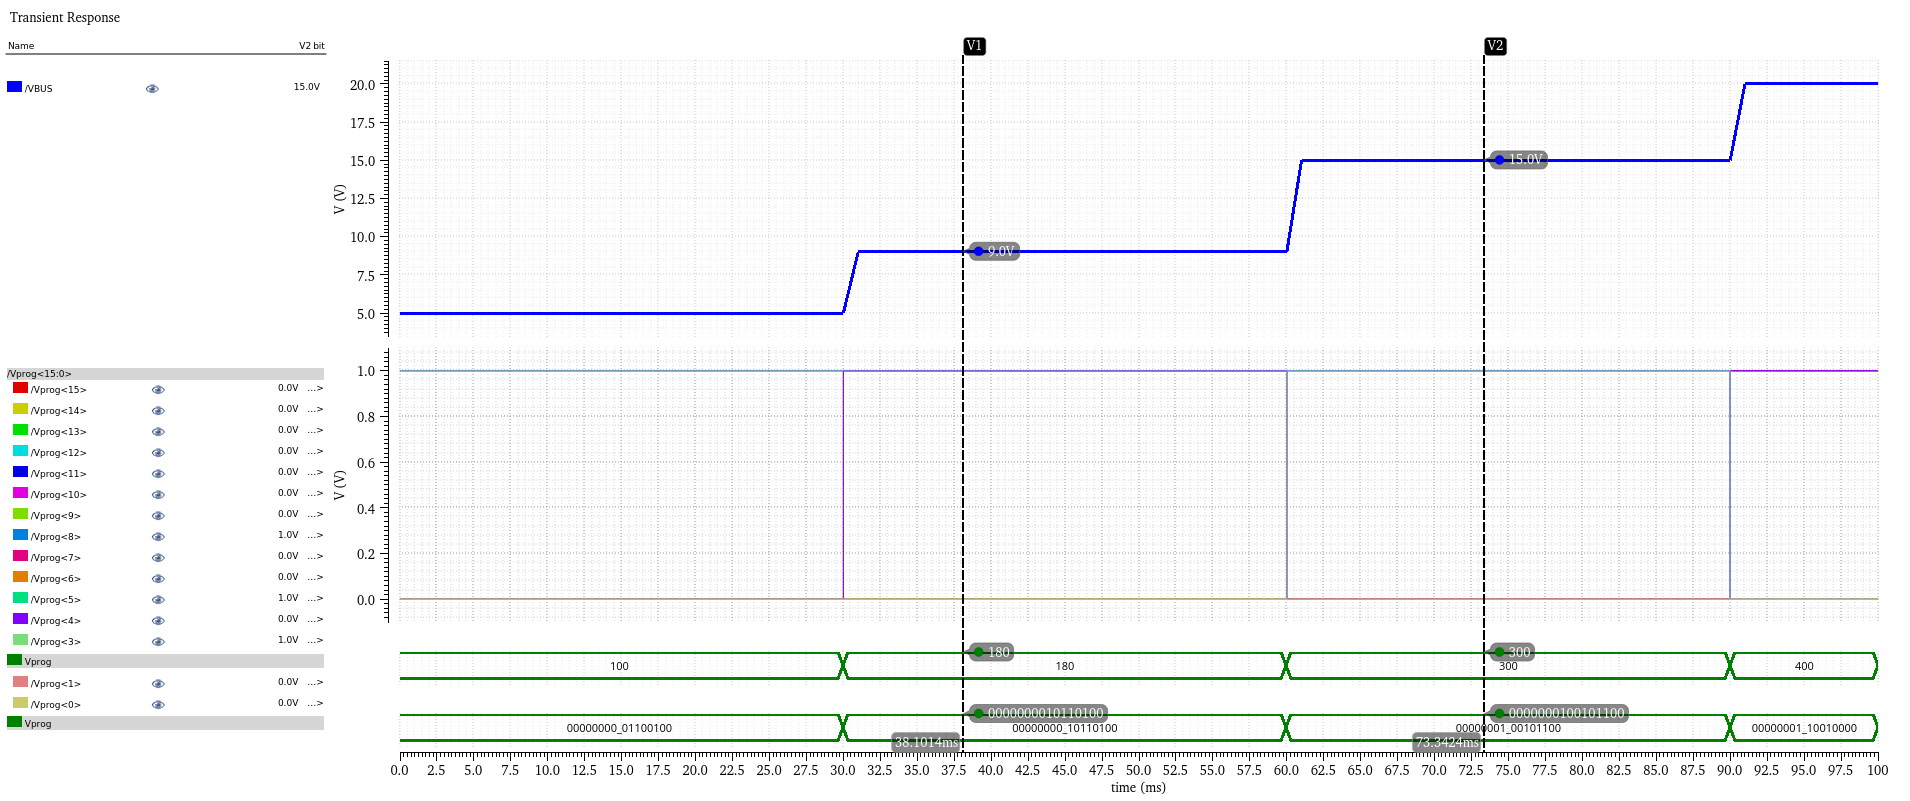
\includegraphics[width=\linewidth]{Chapter5/vs_all.png}
    \caption{Power supply Test - Post Integration}
    \label{fig:ps_all}
\end{figure}

The graph (figure \ref{fig:ps_all}) illustrates the transition response of the power supply’s output voltage, labeled as VBUS, over time. The horizontal axis represents time in milliseconds, ranging from 0 to 175 ms, while the vertical axis shows voltage levels from 0 to 25 V. The blue line on the graph indicates the changes in VBUS, which occur at specific times, demonstrating the system’s ability to adjust the output voltage dynamically.

VBUS is the output voltage of the power supply, which can be adjusted by setting Vprog. Vprog is a 16-bit bus that allows for fine-tuning the output voltage in increments of 50 mV. This granularity ensures precise control over the voltage levels, making the system highly adaptable to various power requirements.

The adjustment of VBUS is managed by a power delivery controller. This controller receives requests from sink devices via CC (Communication Channel) lines. Based on these requests, the controller sets the appropriate value on Vprog, thereby altering the output voltage to meet the specific needs of the connected devices. This mechanism ensures that the power supply can respond quickly and accurately to changes in demand, providing a flexible and efficient power delivery solution.

The ability to fine-tune the output voltage based on external requests makes this system highly flexible. It can cater to a wide range of devices with different power requirements, ensuring optimal performance and energy efficiency. This adaptability is crucial in modern electronics, where devices often have varying power needs and require precise voltage levels for optimal operation.


 \begin{figure}[H]
     \centering
     \begin{tikzpicture}

\begin{axis}[
    title={\textbf{5V to 9V transition, I(load) \approx 5A}},
    xlabel={Time [ms]},
    ylabel={VBUS [volts]},
    xmin=29, xmax=32,
    ymin=5, ymax=10,
    xtick={29,29.5,30,30.5,31,31.5},
    ytick={6,7,8,9,10},
    legend pos=north east,
    ymajorgrids=true,
    grid style=dashed,
]

\addplot[
    color=blue,
    mark=square,
    ]
    coordinates {
    (29,5)(29.25,5)(29.5,5)(29.75,5)(30,5.1)(30.25,5.5)(30.5,6)(30.75,6.5)(31,8.9)(31.25,9.2)(31.5,9.1)(31.75,9.0)(32,9.0)
    };
\end{axis}
\end{tikzpicture}
\hskip 5pt
\begin{tikzpicture}
    \begin{axis}[
    title={\textbf{9V to 15V transition, I(load) \approx 5A}},
    xlabel={Time [ms]},
    ylabel={VBUS [volts]},
    xmin=59, xmax=62,
    ymin=9, ymax=16,
    xtick={59,59.5,60,60.5,61,61.5},
    ytick={9,10,11,12,13,14,15,16},
    legend pos=north east,
    ymajorgrids=true,
    grid style=dashed,
]

\addplot[   color=blue,    mark=square,    ]
    coordinates {    (59,9)(59.25,9)(59.5,9.3)(59.75,10.5)(60,13.1)(60.25,14.5)(60.5,15)(60.75,15.3)(61,14.8)(61.25,15.2)(61.5,14.9)(61.75,15.0)(62,15.0)    };
\end{axis}
\end{tikzpicture}
\begin{tikzpicture}
    \begin{axis}[
    title={\textbf{15V to 20V transition, I(load) \approx 5A}},
    xlabel={Time [ms]},
    ylabel={VBUS [volts]},
    xmin=89, xmax=92,
    ymin=15, ymax=21,
    xtick={89,89.5,90,90.5,91,91.5},
    ytick={16,17,18,19,20,21},
    legend pos=north east,
    ymajorgrids=true,
    grid style=dashed,
]

\addplot[
    color=blue,
    mark=square,
    ]
    coordinates {
    (89,15)(89.25,15)(89.5,15)(89.75,15)(90,15.1)(90.25,15.5)(90.5,16)(90.75,19.5)(91,20.5)(91.25,20.3)(91.5,19.8)(91.75,20.0)(92,20.0)
    };
\end{axis}
\end{tikzpicture}
     \caption{Voltage Transistions}
     \label{fig:enter-label}
 \end{figure}
 
In power supply design, particularly for high-load operations, controlling the voltage slew rate of VBUS is crucial to minimize undesirable effects such as ringing and harmonics. Voltage slew rate refers to the rate at which the output voltage changes over time. By intentionally controlling this rate, the power supply can achieve smoother transitions, reducing the likelihood of oscillations and noise that can interfere with the performance of the system.

Ringing is a phenomenon where oscillations occur due to sudden changes in voltage or current. These oscillations can lead to instability and noise in the power supply, affecting the performance of connected devices. By controlling the voltage slew rate, the power supply can limit the abruptness of voltage transitions, thereby reducing the energy that excites these oscillations. This results in a more stable output voltage with fewer oscillations, ensuring that the power supply delivers clean and reliable power to the load.

Harmonics are higher frequency components that arise from non-linearities in the power supply system. Sudden voltage transitions can generate these harmonics, which can propagate through the system and cause electromagnetic interference (EMI) and signal integrity issues. By controlling the voltage slew rate, the power supply can smooth out these transitions, reducing the generation of harmonics. This helps in maintaining the integrity of the power signal and minimizes EMI, which is critical for the proper functioning of sensitive electronic components.

Overall, controlling the voltage slew rate of VBUS enhances the performance and reliability of the power supply system. It ensures that the output voltage transitions are smooth and controlled, reducing the risk of ringing and harmonic generation. This not only improves the stability and efficiency of the power supply but also ensures that connected devices receive clean and stable power, which is essential for their optimal operation.

The integrated chip undergoes rigorous simulation testing to ensure it meets the specifications set by STMicro and USB compliance standards. Simulation testing is a crucial step in the design and validation process, allowing engineers to verify the functionality and performance of the chip before physical prototypes are manufactured. 

STMicro provides a comprehensive set of specifications and guidelines for testing integrated circuits. These specifications cover various aspects of the chip’s performance, including power management, signal integrity, thermal behavior, and reliability. During simulation testing, the chip is subjected to a series of tests designed to evaluate its compliance with these specifications. For example, power management tests might involve simulating different load conditions to ensure the chip can maintain stable voltage and current outputs. Signal integrity tests might involve analyzing the chip’s response to high-frequency signals to ensure minimal noise and crosstalk. Thermal tests might involve simulating different operating temperatures to ensure the chip can operate reliably under various thermal conditions\cite{st_l4970a}.

In addition to meeting STMicro specifications, the chip must also comply with USB standards. USB compliance testing involves a series of tests designed to ensure the chip can communicate effectively with other USB devices and provide the necessary power delivery. These tests might include evaluating the chip’s ability to handle different data transfer rates, ensuring it can provide stable power to connected devices, and verifying its compliance with USB power delivery protocols. By simulating these scenarios, engineers can ensure the chip meets the stringent requirements of USB standards, providing reliable and efficient performance in real-world applications.

\section{Electromigration and IR Analysis}

\begin{figure}
    \centering
    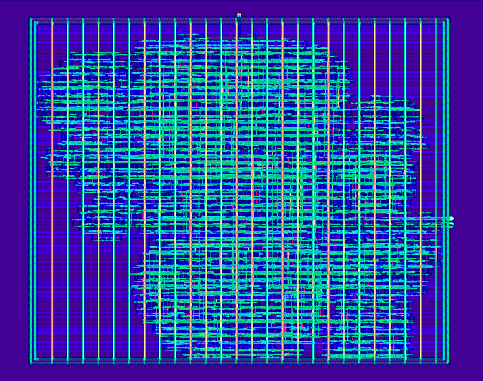
\includegraphics[width=0.6\linewidth]{Chapter5/emir_controller.png}
    \caption{EMIR view of Power Delivery controller}
    \label{fig:emir_pdc}
\end{figure}
EMIR (Electro-Migration and IR-drop) analysis is crucial in the design and verification of integrated circuits, particularly for ensuring the reliability and efficiency of power delivery networks within the chip.

In the figure \ref{fig:emir_pdc}, the background is predominantly purple, overlaid with a grid of thin white lines forming small rectangles. These lines likely represent the layout of the power delivery network. Superimposed on this grid are numerous horizontal and vertical yellow lines, which denote the paths of the power supply network. These lines are densely packed in the central region and become sparser towards the edges, indicating a higher concentration of power delivery paths in the core area of the controller block.

The red spots scattered across the network are of particular interest. These spots indicate areas with high IR (voltage) drop. An IR drop occurs when there is a significant voltage drop across a section of the power delivery network due to high current flow. The presence of these red spots suggests that these regions are experiencing higher electrical activity compared to other areas, leading to a substantial voltage drop.
\begin{figure}
    \centering
    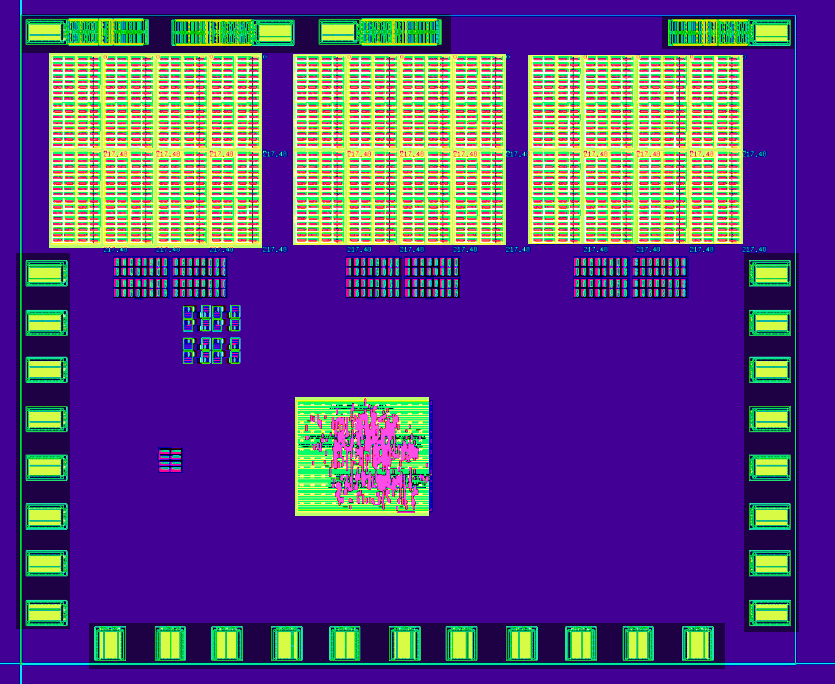
\includegraphics[width=0.6\linewidth]{Chapter5/emir_int_excl.png}
    \caption{EMIR view of Integrated Chip}
    \label{fig:emir_all}
\end{figure}

In the EMIR view of an integrated chip (figure \ref{fig:emir_all}), various components are color-coded to indicate their electrical characteristics and the current they carry. This visualization helps engineers identify potential issues in the power delivery network and optimize the design for better performance and reliability.

Powercells are depicted in yellow in the EMIR view. These components are responsible for carrying large currents, typically around 5A. The yellow color indicates that these cells are handling significant electrical loads, which is crucial for the overall power distribution within the chip. High current-carrying powercells are essential for maintaining stable voltage levels across the chip, ensuring that all parts receive adequate power for proper operation. However, these high currents can also lead to increased IR drops and potential electro-migration issues, making it important to monitor and manage these areas carefully.

The power delivery controller block is shown in green, with some parts highlighted in pink. The green color generally represents areas with moderate current flow and voltage levels, indicating that these regions are functioning within acceptable parameters. However, the pink areas within the power delivery controller block suggest regions with higher electrical activity or potential issues. These pink spots may indicate localized areas of higher current density or voltage drops, which could affect the performance and reliability of the controller block. Engineers need to pay special attention to these pink areas to ensure that the power delivery remains stable and efficient.

IO pins are excluded from the EMIR analysis because their parasitic elements are not extracted. Parasitic elements, such as capacitance, resistance, and inductance, can significantly impact the performance of IO pins, but they are often complex and challenging to model accurately. By excluding IO pins from the analysis, the focus remains on the core components of the power delivery network, allowing for a more straightforward and manageable evaluation of the chip’s power integrity. However, it is still essential to consider the impact of IO pins in the overall design and ensure that they are adequately accounted for in other stages of the design process.

This chapter presents simulation results, focusing on key metrics such as power efficiency, response time, and compliance with USB PD standards. It discusses the challenges encountered during hardware implementation and the solutions devised to address them. The chapter concludes with a critical analysis of the results, discussing their implications.